\section{Modelo entidad-relación}\label{sec:modelo-laura}
\subsection{Del recurso conceptual al almacenamiento}
El modelo distingue cuentas, catálogo y hechos del gimnasio. La Tabla~\ref{tab:puente-laura} relaciona los recursos conceptuales con su implementación. Una categoría identifica un tipo de clase; una etiqueta describe una reseña. Ninguna requiere operaciones independientes en esta API.
\begin{table}[!t]\caption{Correspondencia conceptual y física}\label{tab:puente-laura}\centering\footnotesize
\begin{tabular}{p{.31\columnwidth}p{.59\columnwidth}}\toprule
Recurso & Destino físico \\ \midrule
Usuario & \texttt{users} \\
Clase programada & \texttt{scheduled\_\allowbreak{}classes} \\
Categoría & \texttt{scheduled\_\allowbreak{}classes.category} \\
Paquete de clases & \texttt{packages} \\
Compra & \texttt{purchases} \\
Reserva y asistencia & \texttt{reservations} \\
Reseña & \texttt{reviews} \\
Etiqueta & \texttt{reviews.tags (JSON)} \\
Marca personal & \texttt{personal\_\allowbreak{}records} \\\bottomrule\end{tabular}\end{table}
\subsection{Decisión sobre las siete tablas}
Se mantienen siete tablas porque una reserva, una compra, una reseña y una marca personal representan hechos diferentes. Se evaluó una alternativa de cinco tablas sin \texttt{reservations} ni \texttt{personal\_records}. Se descartó porque no permite controlar el cupo por usuario (RF-05), distinguir reserva y asistencia (RF-06), calcular rachas y totales por categoría (RF-08 y RF-09), ni guardar las marcas personales (RF-10). No se usan las compras o las reseñas como prueba de asistencia.

\subsection{Atributos y claves}
El esquema contiene 49 columnas. Todos los identificadores primarios son enteros autoincrementales. \texttt{users.failed\_login\_attempts} y \texttt{users.locked\_until} representan el contador de intentos fallidos y el fin del bloqueo de la cuenta. La Tabla~\ref{tab:atributos-laura} conserva los nombres físicos, mientras la API utiliza alias como \texttt{id}, \texttt{user\_id} y \texttt{class\_id} al responder.
\begin{table*}[!t]\caption{Siete tablas y sus 49 columnas}\label{tab:atributos-laura}\centering\footnotesize
\begin{tabular}{p{.20\textwidth}p{.74\textwidth}}\toprule
Tabla & Columnas físicas \\ \midrule
\texttt{users} (9) & \texttt{idusers}, \texttt{name}, \texttt{email}, \texttt{password}, \texttt{role}, \texttt{status}, \texttt{registered\_\allowbreak{}at}, \texttt{failed\_\allowbreak{}login\_\allowbreak{}attempts}, \texttt{locked\_\allowbreak{}until} \\
\texttt{scheduled\_\allowbreak{}classes} (9) & \texttt{idscheduled\_\allowbreak{}classes}, \texttt{name}, \texttt{instructor\_\allowbreak{}name}, \texttt{category}, \texttt{price}, \texttt{capacity}, \texttt{starts\_\allowbreak{}at}, \texttt{ends\_\allowbreak{}at}, \texttt{description} \\
\texttt{packages} (5) & \texttt{idpackages}, \texttt{name}, \texttt{price}, \texttt{class\_\allowbreak{}quantity}, \texttt{description} \\
\texttt{purchases} (5) & \texttt{idpurchase}, \texttt{paid\_\allowbreak{}price}, \texttt{purchased\_\allowbreak{}at}, \texttt{idusers}, \texttt{idpackages} \\
\texttt{reservations} (5) & \texttt{idreservation}, \texttt{user\_\allowbreak{}id}, \texttt{class\_\allowbreak{}id}, \texttt{created\_\allowbreak{}at}, \texttt{status} \\
\texttt{reviews} (9) & \texttt{idreview}, \texttt{rating}, \texttt{comment}, \texttt{tags}, \texttt{created\_\allowbreak{}at}, \texttt{updated\_\allowbreak{}at}, \texttt{iduser}, \texttt{idclass}, \texttt{intensity} \\
\texttt{personal\_\allowbreak{}records} (7) & \texttt{idrecord}, \texttt{user\_\allowbreak{}id}, \texttt{exercise}, \texttt{record\_\allowbreak{}type}, \texttt{value}, \texttt{unit}, \texttt{achieved\_\allowbreak{}on} \\
\bottomrule\end{tabular}\end{table*}
\subsection{Relaciones y restricciones}
Cada fila hija pertenece a exactamente un padre en cada relación de la Tabla~\ref{tab:relaciones-laura}; un padre puede tener cero o muchas filas hijas. Las siete claves foráneas son obligatorias y no forman parte de la clave primaria hija. Por tanto, las relaciones son no identificadoras. Las referencias se protegen en InnoDB mediante claves foráneas~\cite{mysql-fk}.
\begin{table*}[!t]\caption{Claves foráneas y cardinalidades}\label{tab:relaciones-laura}\centering\footnotesize
\begin{tabular}{p{.43\textwidth}p{.43\textwidth}p{.07\textwidth}}\toprule
Padre: clave & Hija: referencia & Relación \\ \midrule
\texttt{users.idusers} & \texttt{personal\_\allowbreak{}records.user\_\allowbreak{}id} & 1:0..N \\
\texttt{packages.idpackages} & \texttt{purchases.idpackages} & 1:0..N \\
\texttt{users.idusers} & \texttt{purchases.idusers} & 1:0..N \\
\texttt{scheduled\_\allowbreak{}classes.idscheduled\_\allowbreak{}classes} & \texttt{reservations.class\_\allowbreak{}id} & 1:0..N \\
\texttt{users.idusers} & \texttt{reservations.user\_\allowbreak{}id} & 1:0..N \\
\texttt{scheduled\_\allowbreak{}classes.idscheduled\_\allowbreak{}classes} & \texttt{reviews.idclass} & 1:0..N \\
\texttt{users.idusers} & \texttt{reviews.iduser} & 1:0..N \\
\bottomrule\end{tabular}\end{table*}
El correo es único. También son únicas las parejas de usuario y clase en \texttt{reservations} y \texttt{reviews}; una persona no puede reservar ni reseñar dos veces la misma clase. Los \texttt{CHECK} restringen roles, estados, precios no negativos, cupo positivo, horario coherente, calificación de 1 a 5, intensidad permitida, arreglo de etiquetas y valor positivo de las marcas. La pertenencia de una reseña a una asistencia confirmada se valida en el servicio; no existe una clave foránea de la reseña a la reserva.

\subsection{Valores almacenados y derivados}
\texttt{purchases.paid\_price} describe el precio efectivamente pagado; \texttt{packages.price} describe el catálogo. Los cupos disponibles se obtienen restando las reservas de la capacidad. La racha semanal y los totales por categoría se calculan sobre reservas con estado \texttt{attended}. No se guardan listas de clases dentro de \texttt{users}.

La categoría se normaliza a minúsculas y sin espacios exteriores. Las etiquetas opcionales se guardan como arreglo JSON, con hasta diez cadenas sin duplicados. MySQL valida la representación JSON~\cite{mysql-json}; el servicio valida su contenido. Se acepta este atributo multivaluado para leer y escribir la reseña completa; no se afirma que todas las columnas del modelo cumplan una normalización relacional estricta. El desarrollo de la normalización se integra en su sección correspondiente del informe general.

\subsection{Diagrama físico verificado}
La Fig.~\ref{fig:modelo-laura} se generó a partir de \texttt{information\_schema} en una instancia MySQL creada con \texttt{database/schema.sql}. Presenta las siete tablas, sus 49 columnas y las siete referencias. PK significa clave primaria; FK, clave foránea; AI, autoincremento; UQ, unicidad individual. Las parejas únicas se especifican en el texto anterior. Los archivos editables y los metadatos permiten revisar la correspondencia sin confundir el diagrama con una captura de Workbench.
\begin{figure*}[!t]\centering
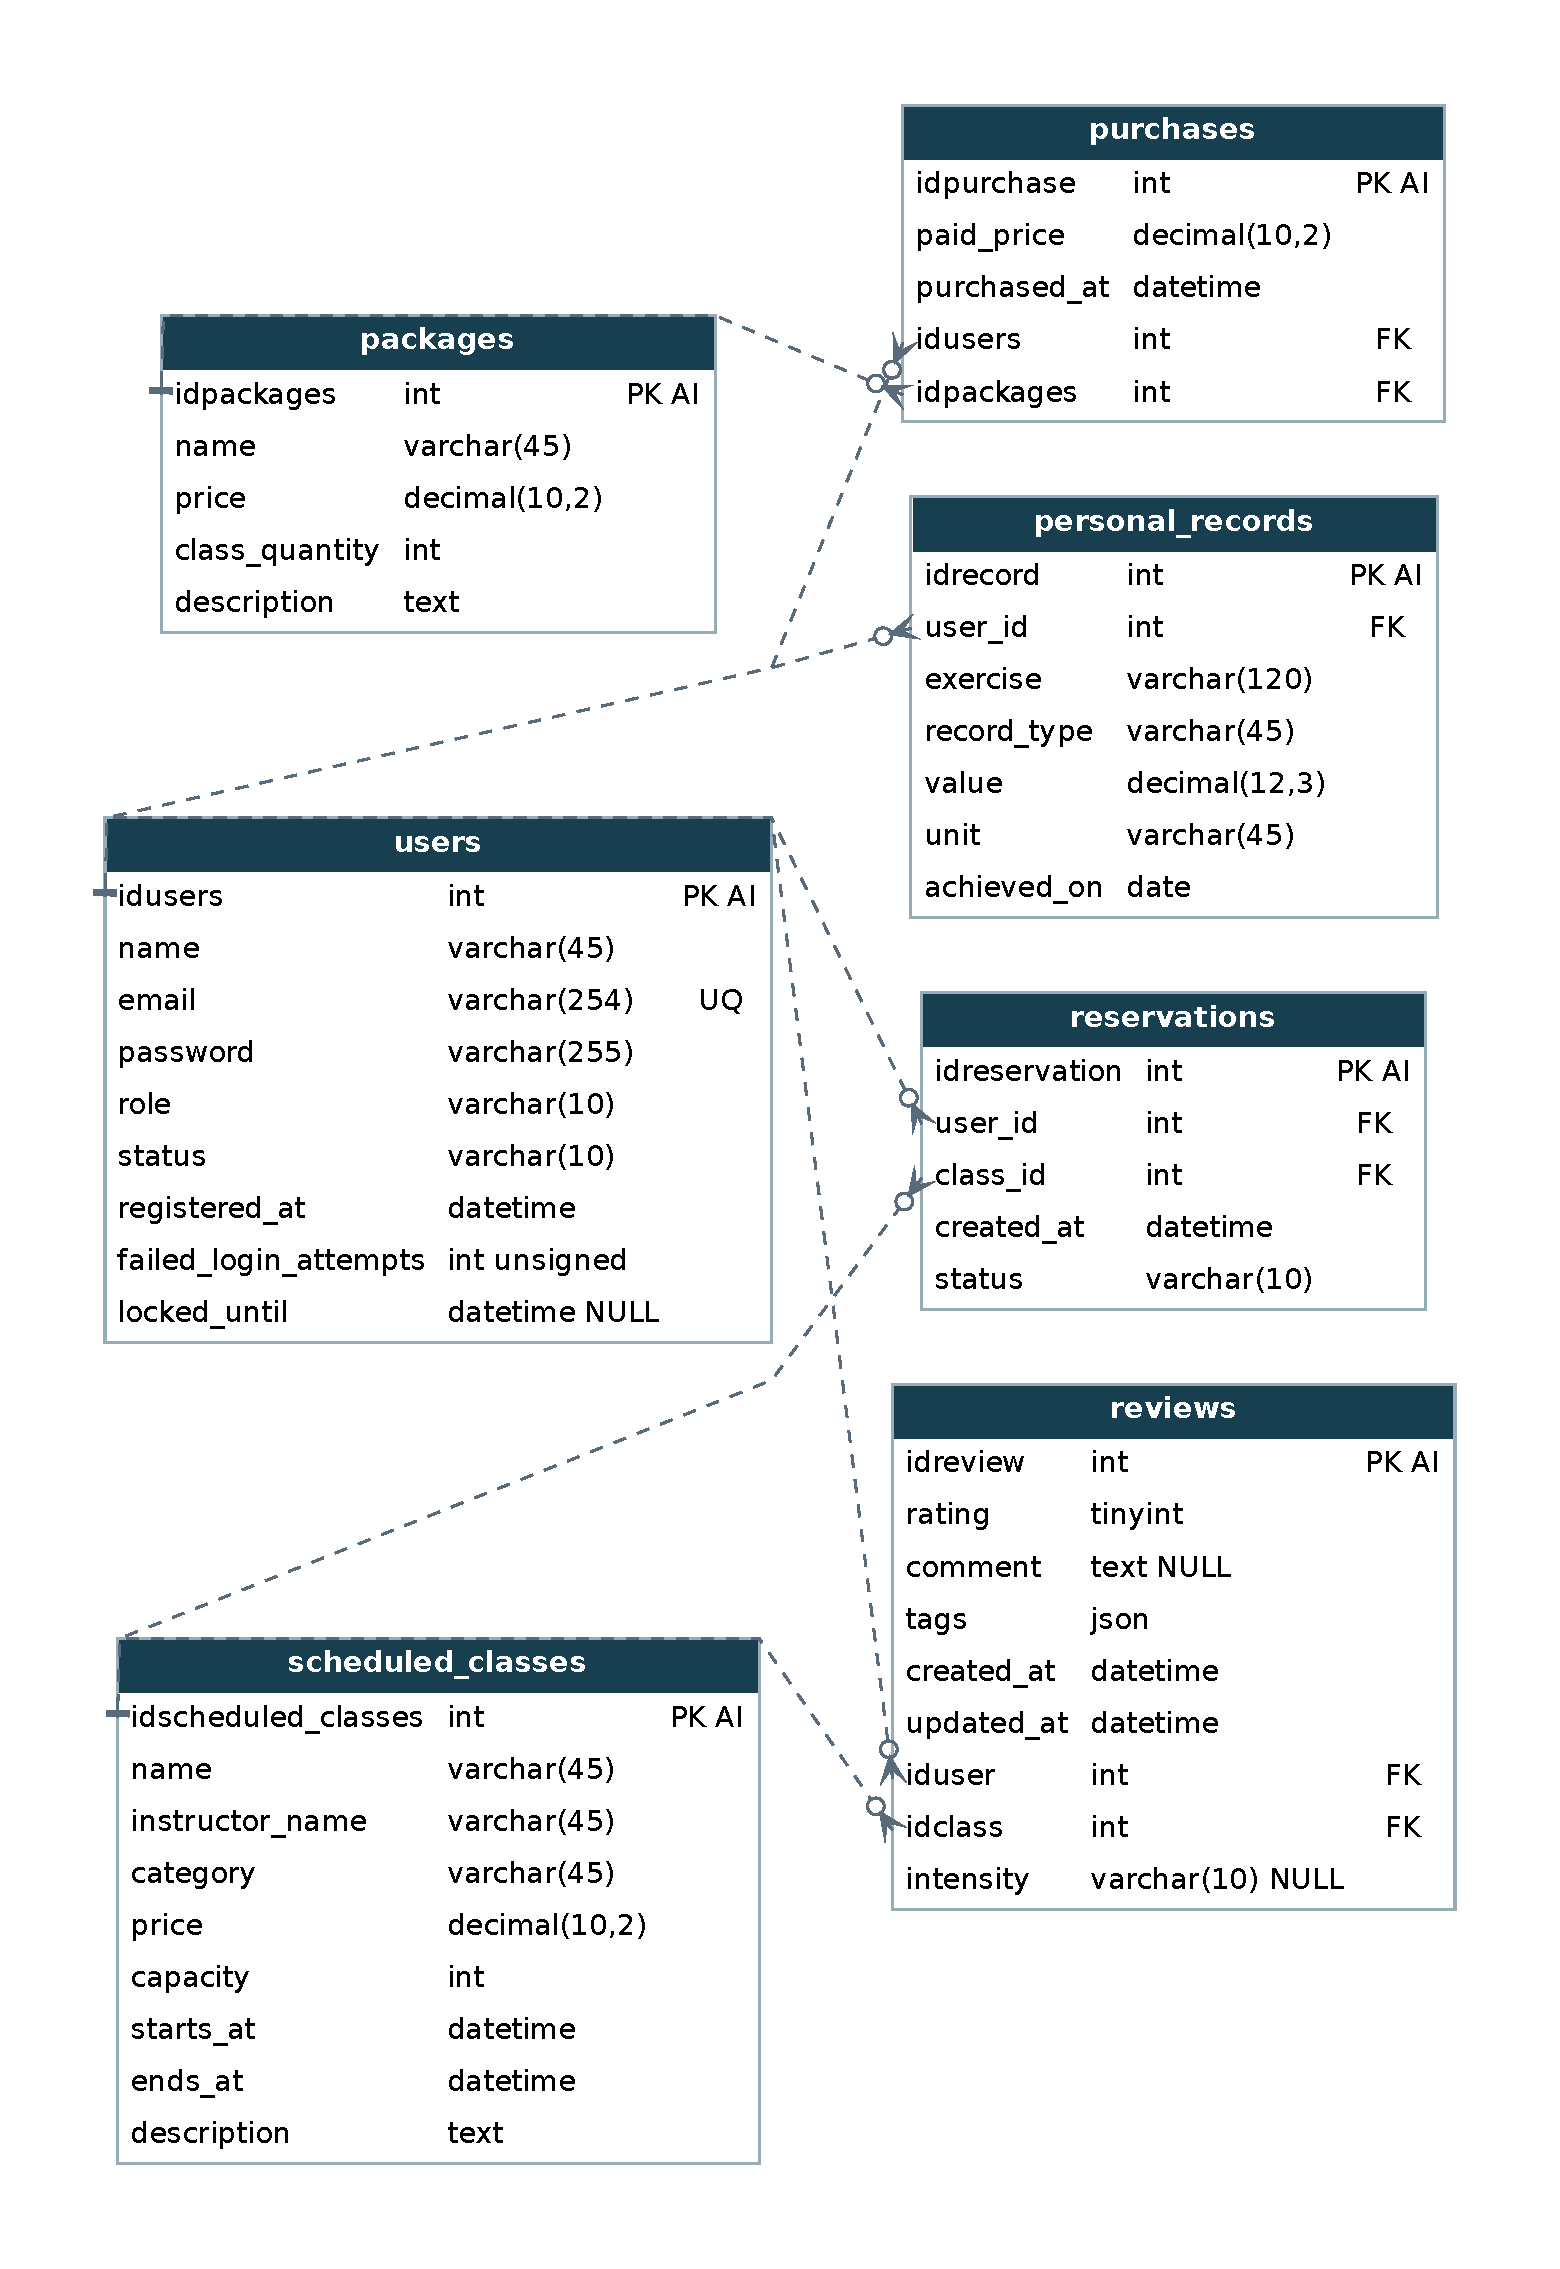
\includegraphics[width=\textwidth,height=.78\textheight,keepaspectratio]{figuras/modelo/modelo-fisico.pdf}
\caption{Modelo físico derivado de los metadatos reales de MySQL. El extremo simple indica un padre; el extremo de círculo y pata de cuervo indica cero o muchos hijos.}\label{fig:modelo-laura}
\end{figure*}
